\section{Introduction}
\label{sec:intro}

Simulation pipelines for embodied artificial intelligence routinely port 3D environments across rendering engines, physics backends, and dataset repositories. During asset ingestion and cross-platform export, proprietary shader graphs authored in NVIDIA Material Definition Language (\textsc{MDL}) within Universal Scene Description (\textsc{USD}) archives are commonly lowered into portable \usdps{} networks. This translation leaves triangle meshes, object poses, articulation hierarchies, camera intrinsics, and language goals untouched. Geometrically, the converted scene appears exact; visually, surface reflectance, specular highlights, glass transmission, local edge contrast, and indirect illumination shift together. Quantifying how this routine conversion alters Vision-Language Model (\textsc{VLM}) decisions is essential before converted assets can be relied upon in evaluation or sim-to-real pipelines.

Benchmarking converted assets by dataset-level accuracy alone hides a critical reliability failure. In many scenes, degraded glass highlights or flattened surface texture cause a model to miss targets it previously grounded, while a comparable number of glare-occluded metallic objects become easier to localize. Their net difference nearly cancels in aggregate accuracy ($+0.42\%$ on \textsc{Qwen3-VL-32B}, \textsc{Molmo2-8B}, and \textsc{LLaVA-NeXT-Mistral-7B}), even as $4.17\%$ to $23.13\%$ of individual task outcomes reverse between conditions. For safety-critical inspection and downstream closed-loop embodied control, silent regression on previously solved instances cannot be offset by incidental improvements elsewhere.

\begin{figure*}[!t]
\centering
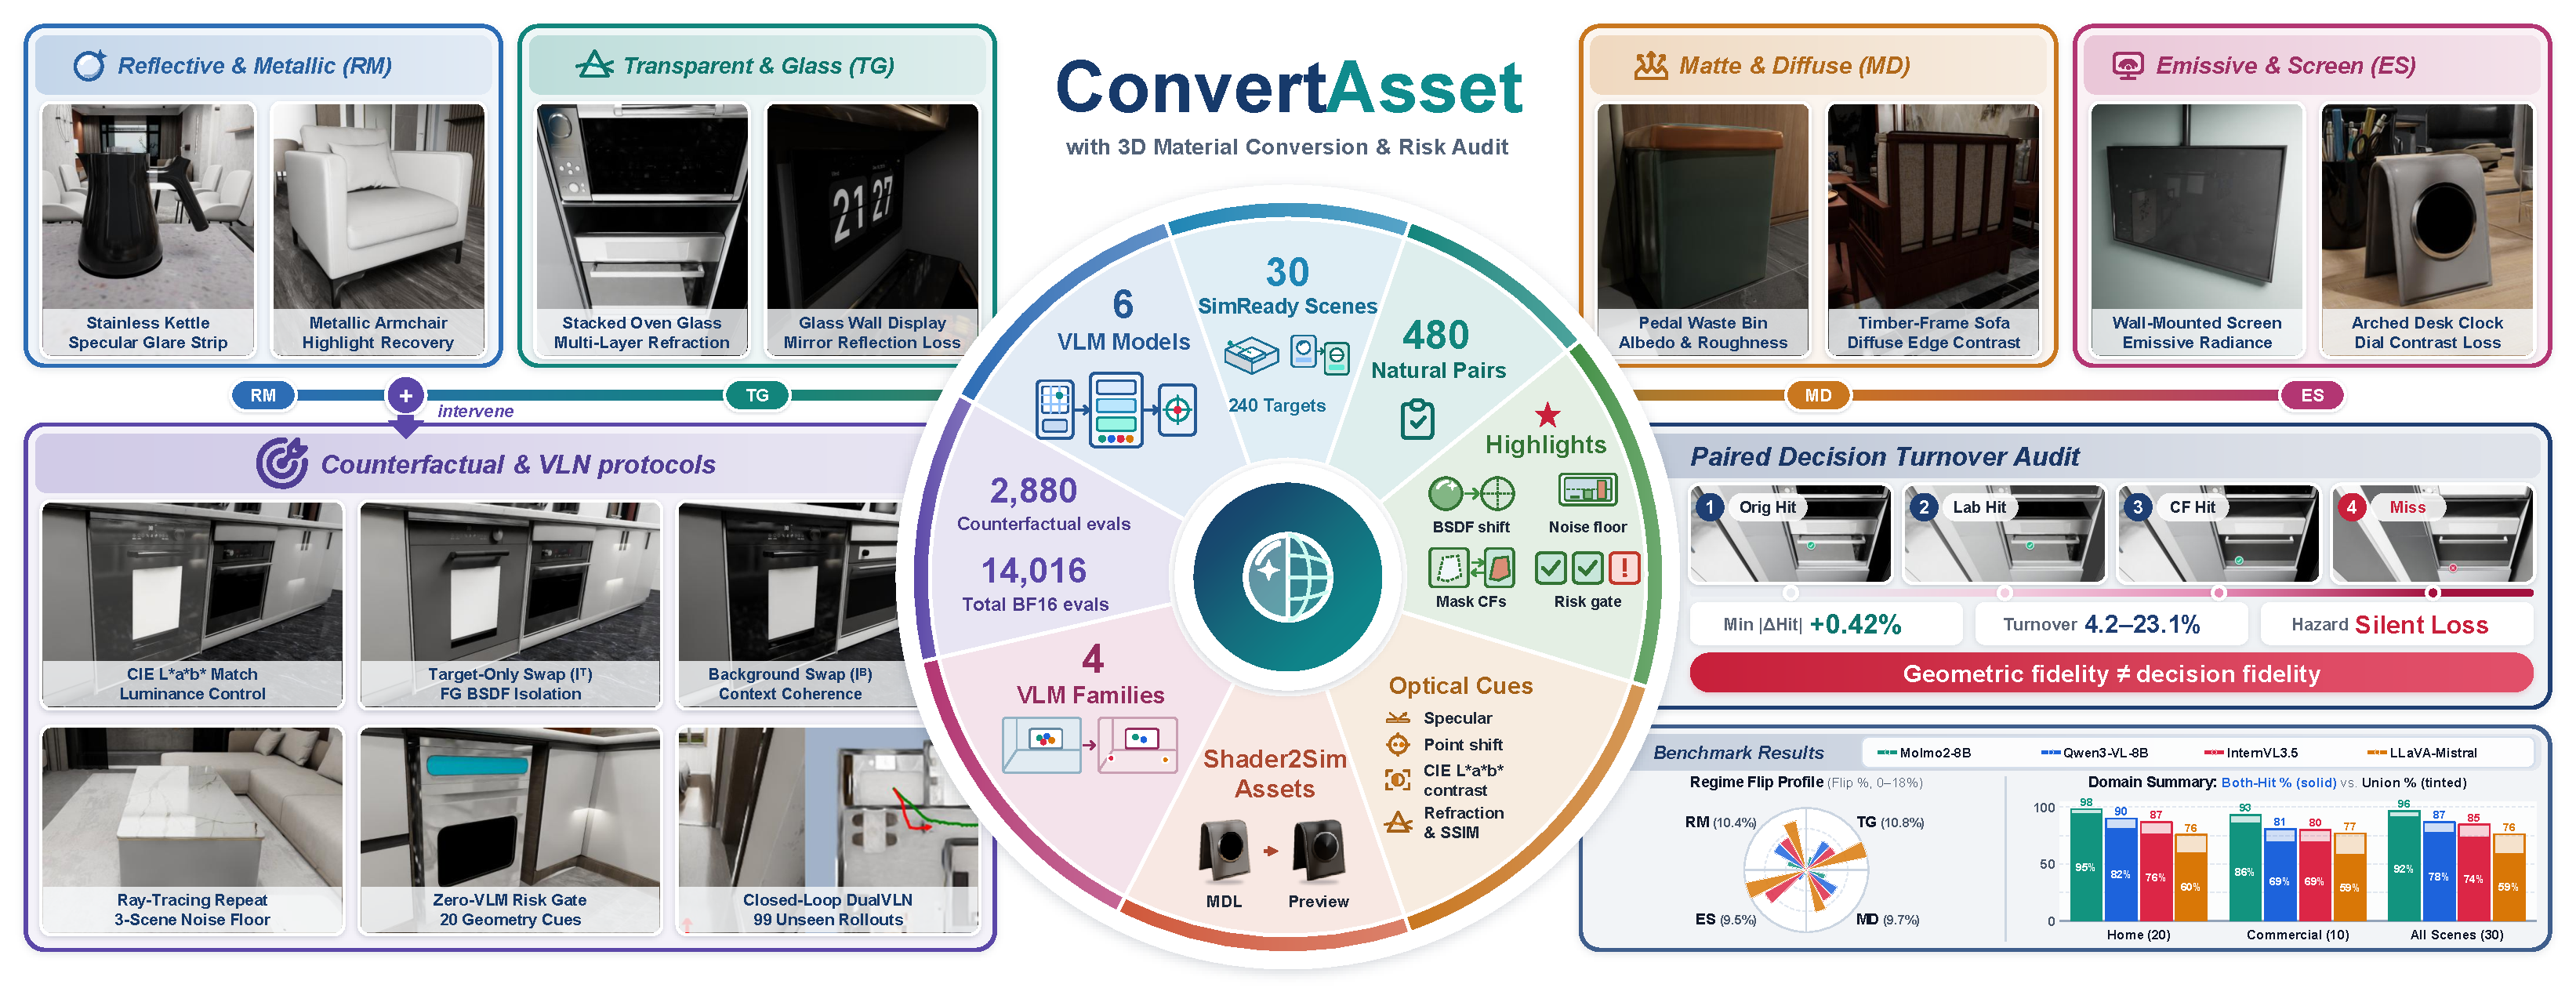
\includegraphics[width=\textwidth]{fig1_overview.pdf}
\caption{\textbf{Overview of the \textsc{ConvertAsset} benchmark, optical domain taxonomy, counterfactual protocols, and four-family audit.}
Across 30 geometry-locked SimReady scenes (240 targets, 480 natural pairs) and four open-weight \textsc{VLM} families under deterministic inference, lowering NVIDIA \textsc{MDL} shaders to \texttt{UsdPreviewSurface} induces $4.2\text{--}23.1\%$ bidirectional pass/fail decision turnover despite small marginal hit-rate deltas ($\min |\Delta H| = +0.4\%$). \emph{Top corners:} paired optical examples spanning Reflective \& Metallic (\textsc{RM}), Transparent \& Glass (\textsc{TG}), Matte \& Diffuse (\textsc{MD}), and Emissive \& Screen (\textsc{ES}). \emph{Bottom:} pixel-exact counterfactual protocols (2,880 evaluations), zero-\textsc{VLM} risk gate, 99 closed-loop \textsc{VLN} episodes, and four-family regime flip profiles and consistency gaps.}
\label{fig:overview}
\end{figure*}

Three methodological gaps limit prior robustness work when applied to 3D asset conversion (Section~\ref{sec:related}). First, classical corruption benchmarks apply 2D post-processing noise or style transfer \citep{Geirhos2019Texture,Hendrycks2019Benchmarking}, whereas generative editing benchmarks modify object silhouettes alongside surface appearance \citep{Zhang2024ImageNetD}. Second, spatial grounding evaluations frequently entangle appearance sensitivity with coordinate-frame mismatches (pixels vs.\ normalized $0\text{--}1000$ outputs), decoding randomness \citep{Zhao2021Calibrate}, and path-tracing noise, obscuring whether shader effects exceed runtime variance. Third, conventional pixel metrics such as global \textsc{RGB MAE} penalize helpful glare reduction symmetrically with damaging contrast loss, offering little guidance on which converted scenes merit manual inspection.

Figure~\ref{fig:overview} outlines our end-to-end empirical framework. Within \textsc{ConvertAsset}, we hold scene graphs, meshes, transforms, and camera viewpoints identical between \textsc{MDL} (\original) and \usdps{} (\converted) renders across 30 indoor scenes (20 residential, 10 commercial; 240 visible target instances across 480 camera views). Using calibrated deterministic readout protocols validated via an independent coordinate-format qualification step (\ref{app:readout}), we examine four open-weight \textsc{VLM} families (\textsc{Qwen3-VL}, \textsc{InternVL3.5}, \textsc{Molmo2}, and \textsc{LLaVA-NeXT-Mistral}) along four axes:
\begin{itemize}
    \item \textbf{RQ1 (Variance Floor, Scaling, and Four-Family Generality):} Does material-induced bidirectional turnover exceed greedy runtime repeatability and path-tracing variance across all six checkpoints, a $16\times$ parameter span (\textsc{Qwen3-VL-2B/8B/32B}), and four distinct architectures?
    \item \textbf{RQ2 (Cross-Family Causal Optical Mechanisms):} Across 2,880 pixel-exact silhouette counterfactuals and $\mathrm{CIE}~L^*a^*b^*$ photometric controls on two independent 8B architectures, how much turnover arises from overall luminance and color shifts versus non-photometric Bidirectional Scattering Distribution Function (\textsc{BSDF}) structure?
    \item \textbf{RQ3 (Pre-Deployment Risk Gating):} Can lightweight target-geometry and paired-render cues flag conversion regressions prior to running any \textsc{VLM}, outperforming global \textsc{RGB MAE}, and how does cross-architecture regression divergence affect family-specific versus pooled risk gates?
    \item \textbf{RQ4 (Downstream Embodied Control):} How does paired material conversion manifest in sequential closed-loop Vision-and-Language Navigation (\textsc{VLN}) over 99 unseen apartment episodes?
\end{itemize}

\paragraph{Summary of contributions}
\begin{enumerate}
    \item \textbf{Four-Family Asset-Conversion Benchmark and Noise Floor (Sections~\ref{sec:method}--\ref{sec:grounding}):} Across 14,016 deterministic predictions spanning 4 \textsc{VLM} families and 6 checkpoints over 30 scenes, small marginal deltas ($+0.42\%$ on 32B, \textsc{Molmo2-8B}, and \textsc{LLaVA-NeXT}) conceal $4.17\%\text{--}23.13\%$ bidirectional flips. Greedy repeatability stays at $0.00\%$ ($0.00\,\mathrm{px}$) on every checkpoint, whereas shader conversion exceeds same-material ray-tracing variance by $2.00\times$ to $6.00\times$ ($4.17\%$ vs.\ $0.00\%$ on \textsc{Molmo2-8B}).
    \item \textbf{Cross-Family Causal Silhouette Counterfactuals (Section~\ref{sec:mechanisms}):} Across 2,880 counterfactual evaluations on \textsc{Qwen3-VL-8B} and \textsc{InternVL3.5-8B-HF}, both architectures retain an identical \textbf{$+3.54\%$} non-photometric shader residual above $\mathrm{CIE}~L^*a^*b^*$ salience matching ($+3.38\%$ on the 473 bit-identical mask subset), reflecting glare cleanup on metallic objects balanced against glass and texture degradation.
    \item \textbf{Family-Calibrated vs.\ Pooled Risk Gating (Section~\ref{sec:risk_gate}):} An $\ell_2$-regularized logistic gate combining target geometry with paired appearance deltas reaches $0.743$ held-out test \textsc{AUROC} ($0.732$ 30-scene \textsc{LOSO}) on \textsc{Qwen3-VL} regressions, capturing $52.0\%$ of \textsc{LOSO} losses within a $20\%$ inspection budget where global \textsc{RGB MAE} yields $0.432$. Finding that $85.7\%$ ($66/77$) of $\ge$7B losses are unique to a single architecture further explains why pre-deployment gates must be calibrated per model family ($0.582$ test / $0.536$ \textsc{LOSO} when pooled).
    \item \textbf{Downstream Closed-Loop Context and Analysis Suite (Section~\ref{sec:navigation}):} We extend the static grounding analysis with 99 paired closed-loop \textsc{InternNav/\allowbreak DualVLN} episodes showing $30.3\%$ episode-outcome turnover, alongside a complete set of scene renders, mask counterfactuals, and diagnostic scripts.
\end{enumerate}

\paragraph{Relation to preliminary workshop work}
A preliminary workshop study introducing the underlying conversion toolkit appeared in \citet{Zhu2026Evaluating}, focusing on single-asset image similarity (\textsc{PSNR}, \textsc{SSIM}, \textsc{LPIPS}), feature cosines (\textsc{CLIP}, \textsc{DINOv2}), and simulator warm-up timing. Over $85\%$ of the present article is new, contributing the 30-scene \textsc{ConvertAsset} grounding benchmark, 14,016 four-family \textsc{VLM} evaluations, the four-level variance hierarchy, 2,880 silhouette counterfactuals, family-calibrated zero-\textsc{VLM} risk gating, and the 99-episode closed-loop navigation study.
